% Use only LaTeX2e, calling the article.cls class and 12-point type.

\documentclass[12pt]{article}

% Users of the {thebibliography} environment or BibTeX should use the
% scicite.sty package, downloadable from *Science* at
% http://www.sciencemag.org/authors/preparing-manuscripts-using-latex 
% This package should properly format in-text
% reference calls and reference-list numbers.

\usepackage{scicite}

\usepackage{times}

% The preamble here sets up a lot of new/revised commands and
% environments.  It's annoying, but please do *not* try to strip these
% out into a separate .sty file (which could lead to the loss of some
% information when we convert the file to other formats).  Instead, keep
% them in the preamble of your main LaTeX source file.


%%%%%% taken from papaja-created ver
\usepackage{csquotes}
\usepackage{graphicx}
  \usepackage[unicode=true]{hyperref}
  
% The following parameters seem to provide a reasonable page setup.

\topmargin 0.0cm
\oddsidemargin 0.2cm
\textwidth 16cm 
\textheight 21cm
\footskip 1.0cm


%The next command sets up an environment for the abstract to your paper.

\newenvironment{sciabstract}{%
\begin{quote} \bf}
{\end{quote}}



% Include your paper's title here

\title{Polite speech arises from desires to be helpful and look helpful} 


% Place the author information here.  Please hand-code the contact
% information and notecalls; do *not* use \footnote commands.  Let the
% author contact information appear immediately below the author names
% as shown.  We would also prefer that you don't change the type-size
% settings shown here.

\author
%{Erica J. Yoon,$^{1\ast}$ Michael Henry Tessler,$^{1\ast}$ Noah D. Goodman,$^{1}$ Michael C. Frank$^{1}$\\
%\\
%\normalsize{$^{1}$Department of Psychology, Stanford University}\\
%\\
%\normalsize{$^\ast$These authors contributed equally to this work.}
%
%}
{Erica J. Yoon,$^{1\ast\dagger}$ Michael Henry Tessler,$^{1\ast}$ Noah D. Goodman,$^{1}$ Michael C. Frank$^{1}$\\
\\
\normalsize{$^{1}$Department of Psychology, Stanford University,}\\
\normalsize{450 Serra Mall, Stanford, CA 94305.}\\
\\
\normalsize{$^\ast$These authors contributed equally to this work.}
\\
\normalsize{$^\dagger$To whom correspondence should be addressed; E-mail: ejyoon@stanford.edu.}
}

% Include the date command, but leave its argument blank.

\date{}



%%%%%%%%%%%%%%%%% END OF PREAMBLE %%%%%%%%%%%%%%%%



\begin{document} 

% Double-space the manuscript.

\baselineskip24pt

% Make the title.

\maketitle 



% Place your abstract within the special {sciabstract} environment.

\begin{sciabstract}
Conveying information in a false or indirect manner in consideration of
listeners' wants (i.e.~being polite) seemingly contradicts an important
goal of communication: information transfer. We model production
of polite speech in which speakers deviate from being maximally
informative for social reasons. We show that speakers produce polite
speech due to their desires to be helpful -- both epistemically (convey
the true state to the listener) and socially (make the listener feel
good) -- and to \emph{appear} helpful. We formalize this tradeoff
between speaker's goals within a probabilistic model and show the model
is able to predict people's polite speech production judgments. Our
extension of formal language modeling frameworktheories of language to account for speakers' social
goals represents an advance in understanding of human speech.
\end{sciabstract}



% In setting up this template for *Science* papers, we've used both
% the \section* command and the \paragraph* command for topical
% divisions.  Which you use will of course depend on the type of paper
% you're writing.  Review Articles tend to have displayed headings, for
% which \section* is more appropriate; Research Articles, when they have
% formal topical divisions at all, tend to signal them with bold text
% that runs into the paragraph, for which \paragraph* is the right
% choice.  Either way, use the asterisk (*) modifier, as shown, to
% suppress numbering.


Human speech is an important means of exchanging information, but
intriguingly it often deviates from maximally efficient and accurate
information transfer. Instead of saying the most direct message that the
speaker wants the listener to access (\enquote{I know for a fact that
you failed the exam}; \enquote{Tell me where Jordan Hall is}), Speakers produce
vague or underinformative remarks (\enquote{I don't think you did very
well on the exam}) or add extraneous, seemingly irrelevant markers
(\enquote{\emph{could you please} tell me where Jordan Hall is?}). People sometimes
even produce false utterances that completely misrepresents the
speaker's knowledge (\enquote{Your talk was great!} about a truly
terrible talk).

Polite language, in which speakers convey information in a false or
indirect manner in consideration of listeners' wants, violates a
critical principle of cooperative communication: exchanging information
efficiently and accurately \cite{grice1975}. Yet polite speech serves
another important goal of communication: maintaining and improving
social relationships. Here we propose that cooperative communication
reflects a principled tradeoff between two goals: epistemic goal, or to
convey information accurately and efficiently; and social goal, or to
make the interactants feel good.

How can we model production of polite speech? The Rational Speech Act
(RSA) framework describes language understanding as recursive
probabilistic inference between a pragmatic listener and an informative
speaker \cite{goodman2016}. This framework has been successful at capturing the
quantitative details of a number of language understanding tasks but it
neglects the social goals a speaker may pursue. On the other hand,
informal theories of politeness explain how speakers' social goals give
rise to polite speech. For example, Brown and Levinson \cite{brown1987} argue that
deviation from informativity increases the level of polite face-saving.
But there has been no formalization of the notion of speakers' social
goals, thus no systemic quantitative predictions of politeness theories
have been available.

We propose a computational model of polite speech (\textbf{pRSA}) that
accounts for both epistemic and social goals of speakers. RSA models
assume speakers choose utterances approximately optimally given a
utility function \cite{goodman2013}. In our model, the
speaker's utility function can be decomposed into two components: First,
\emph{epistemic utility} refers to the standard, informative utility in
RSA: the amount of information a literal listener (\(L_0\)) would still
not know about world state s after hearing a speaker's utterance \(w\).
Second, \emph{social utility} is the expected subjective utility of the
state inferred given the utterance \(w\). The expected subjective
utility is related to the intrinsic value of the state, and we use a
value function (\(V\)) to map states to subjective utility values. This
captures the affective consequences for the listener of being in state
\(s\). The utility weight (single mixture parameter \(\phi_{S_1}\))
determines how informative versus social the speaker wants to be: a
higher \(\phi_{S_1}\) signifies the epistemic goal prioritized over the
social goal. Finally, some utterances might be costlier than others. The
utility of an utterance subtracts the cost \(c(w)\) from the weighted
combination of the social and epistemic utilities.
\[U(w; s; \phi]) = \phi_{S_1}\ \cdot L_0(s \mid w) + 
(1 - \phi_{S_1}) \cdot V[L_0(s \mid w)]  - C(w)\]

The recursive reasoning in our model unfolds as follows: The speaker
(\(S_1\)) in pRSA chooses utterances \(w\) softmax-optimally given the
state \(s\) and his goal mixture parameter weight \(\phi\). Given the
speaker's utterance, the pragmatic listener (\(L_1\)) jointly infers the
state \(s\) and the utility weight \(\phi_{S_1}\). Finally, the
pragmatic speaker (\(S_2\)) chooses an utterance, based on the pragmatic
listener \(L_1\)'s model and one of three possible different goals he
can have: (1) true epistemic goal to convey the true state
(\(\phi_{epistemic}\)); (2) true social goal to make L1 feel good
(\(\phi_{social}\)); (3) self-presentational goal to convey a certain
\(\phi_{S_1}\) to \(L_1\) (i.e.~to \emph{appear} informative or kind;
\(\phi_{self}\)). \[P_{S_2}(w \mid s, \hat{\beta})\propto 
\mathrm{exp}( \phi_{epistemic}\ \cdot L_1(s \mid w) +
\phi_{social}\ \cdot V[L_1(s \mid w)] + 
\phi_{self}\ \cdot L_1(\phi_{S_1} \mid w) )\]

We used a simple procedure to empirically test whether our model is able
to predict production of polite utterances. Participants read scenarios
in which someone (e.g.~Ann) gave a performance of some kind, and another
person (Bob) evaluated it. We provided information on Ann's feelings
toward the presentation (\emph{true state}), which were shown on a scale
from zero to three hearts (e.g.~two out of three hearts filled in red
color; see Figure 1). We also presented Ann's goal, which was one of the
following: (1) to be \emph{informative} and give accurate feedback; to
be \emph{social} and to make Bob feel good; or to be \emph{both}
informative and social at the same time. We hypothesized that speakers
with both goals to be informative and social given bad true states
(i.e.~Bob's performance was poor) would produce more negation
(\enquote{It wasn't\textasciitilde{}}) to save the listener's face while
vaguely conveying the bad true state (see our pre-registered model,
hypothesis, and procedure at FIXME). Each participant read 12 scenarios
total (4 true states \(\times\) 3 goals).

In a single trial, each scenario was followed by a question that asked
for the most likely utterance by Ann. Participants indicated their
answer by choosing one of the options on the two dropdown menus,
side-by-side, one for choosing between \emph{It was} vs. \emph{It
wasn't} and the other for choosing among \emph{terrible}, \emph{bad},
\emph{okay}, \emph{good}, and \emph{amazing}, thereby selecting one of
ten possible utterances (see Figure 1). We separately gathered the
literal meanings of the ten possible utterances, by measuring how likely
each utterance is to be true given each true state, to set expected
literal meanings of utterances in our model (see Supplementary Materials
for literal semantic results).

\begin{figure}
\centering
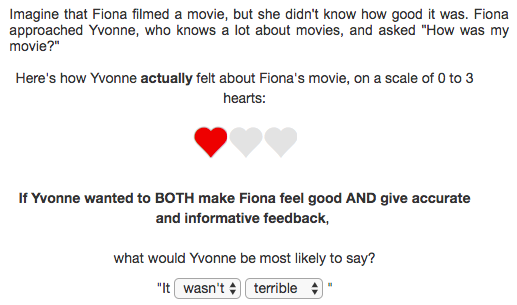
\includegraphics{fig/screenshot.png}
\caption{Example of a trial in the speaker production task.}
\end{figure}

\hypertarget{results}{%
\section{Results}\label{results}}

\begin{figure}
\centering
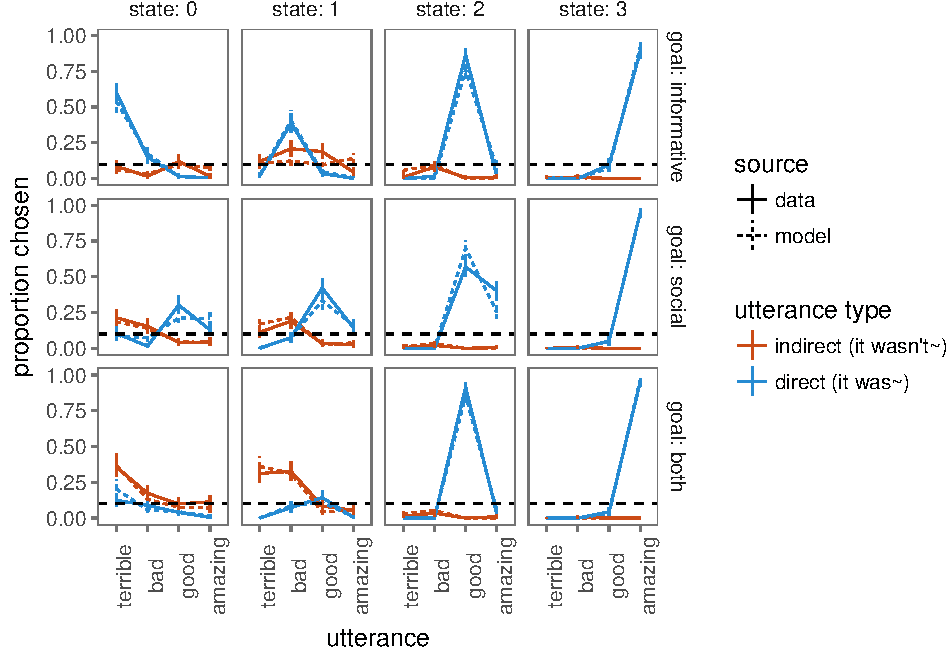
\includegraphics{politeness_files/figure-latex/utterancePrediction-1.pdf}
\caption{\label{fig:utterancePrediction}Experimental results (solid lines)
and fitted model predictions (dashed lines) for speaker production.
Proportion of utterances chosen (utterance type -- direct vs.~indirect
-- in different colors and words shown on x-axis) given the true states
(columns) and speaker goals (rows). Error bars represent 95\% confidence
intervals for the data and 95\% highest density intervals for the model.
Black dotted line represents the chance level.}
\end{figure}

\begin{figure}
\centering
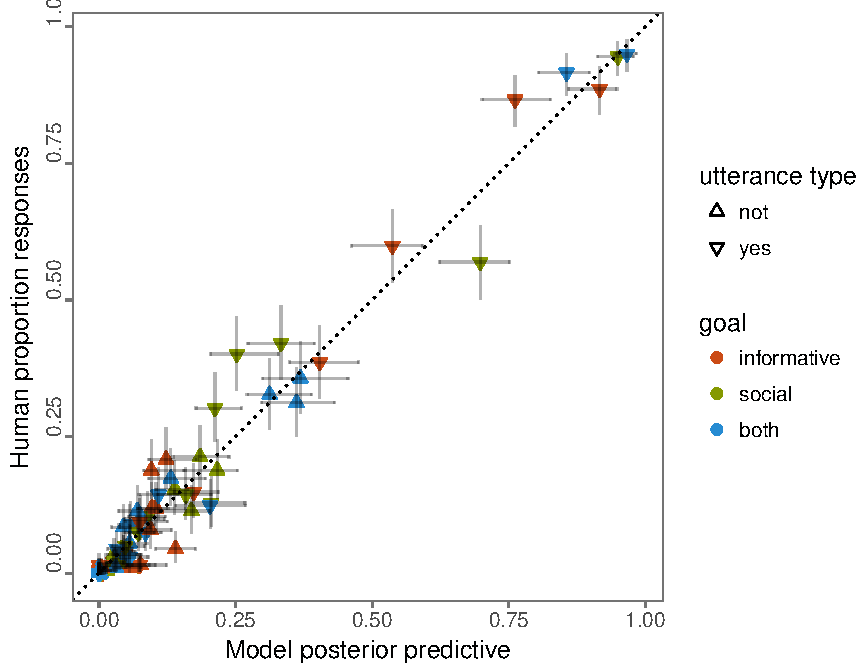
\includegraphics{politeness_files/figure-latex/varianceExplained-1.pdf}
\caption{\label{fig:varianceExplained}Full distribution of human responses
vs.~model predictions. Error bars represent 95\% confidence intervals
for the data (vertical) and 95\% highest density intervals for the model
(horizontal).}
\end{figure}

\begin{figure}
\centering
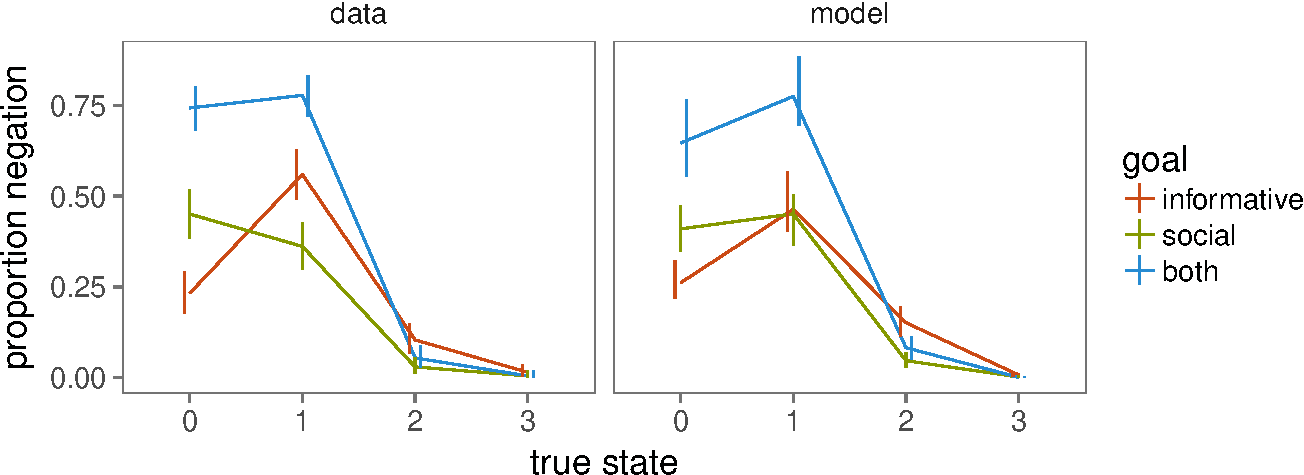
\includegraphics{politeness_files/figure-latex/negationPrediction-1.pdf}
\caption{\label{fig:negationPrediction}Experimental results (left) and
fitted model predictions (right) for average proportion of negation
produced among all utterances, given true states (x-axis) and goals
(colors).}
\end{figure}

Mean proportion of utterances chosen by participants in each true-state
\(\times\) goal condition were overall highly consistent with the our
model predictions (Figure \ref{fig:utterancePrediction}). The posterior
predictive of the model explained almost all of the variance in the
production data \(r^2\)(96) = 0.97 (Figure \ref{fig:varianceExplained}).
Consistent In line with our hypothesis, the both-goal speaker \(\times\)
bad true state (0 or 1 heart) conditions yielded the greatest proportion
of negation (\enquote{It wasn't \textasciitilde{}}; see Figure
\ref{fig:negationPrediction}).

Our work unifies previous formal models of communication and informal
theories of social uses of language. Our findings suggest that neither
epistemic nor social motives alone motivate polite speech; instead,
production of polite speech results from the conflict between these two,
combined with a self-presentational desire to \emph{look} epistemically
and socially helpful. These findings provide strong support for a
utility-theoretic framing of politeness, and suggest new directions in
understanding of pragmatic language use in social contexts.

% Your references go at the end of the main text, and before the
% figures.  For this document we've used BibTeX, the .bib file
% scibib.bib, and the .bst file Science.bst.  The package scicite.sty
% was included to format the reference numbers according to *Science*
% style.

%BibTeX users: After compilation, comment out the following two lines and paste in
% the generated .bbl file. 

\bibliography{politeness}

\bibliographystyle{Science}





\section*{Acknowledgments}
This work was supported by NSERC PGS Doctoral scholarship PGSD3-454094-2014 to EJY, NSF Graduate Research Fellowship DGE-114747 to MHT, ONR grant N00014-13-1-0788 to NDG, and NSF grant BCS 1456077 to MCF.

%Here you should list the contents of your Supplementary Materials -- below is an example. 
%You should include a list of Supplementary figures, Tables, and any references that appear only in the SM. 
%Note that the reference numbering continues from the main text to the SM.
% In the example below, Refs. 4-10 were cited only in the SM.     
\section*{Supplementary materials}
Materials and Methods\\
Supplementary Text\\
Figs. S1 to S3\\
Tables S1 to S4\\
References \textit{(4-10)}


% For your review copy (i.e., the file you initially send in for
% evaluation), you can use the {figure} environment and the
% \includegraphics command to stream your figures into the text, placing
% all figures at the end.  For the final, revised manuscript for
% acceptance and production, however, PostScript or other graphics
% should not be streamed into your compliled file.  Instead, set
% captions as simple paragraphs (with a \noindent tag), setting them
% off from the rest of the text with a \clearpage as shown  below, and
% submit figures as separate files according to the Art Department's
% instructions.


\clearpage

\noindent {\bf Fig. 1.} Please do not use figure environments to set
up your figures in the final (post-peer-review) draft, do not include graphics in your
source code, and do not cite figures in the text using \LaTeX\
\verb+\ref+ commands.  Instead, simply refer to the figure numbers in
the text per {\it Science\/} style, and include the list of captions at
the end of the document, coded as ordinary paragraphs as shown in the
\texttt{scifile.tex} template file.  Your actual figure files should
be submitted separately.

\end{document}




















